%!TEX root = ../synopsis.tex

\thispagestyle{empty}
\noindent
Работа выполнена
на кафедре
<<Информационные технологии и автоматизация проектирования>>
Института новых материалов и технологий
ФГАОУ ВО
<<Уральский федеральный университет имени первого Президента России Б.Н.~Ельцина>>

\vspace{0.008\paperheight plus1fill}

\noindent%
\begin{tabularx}{\textwidth}{@{}lX@{}}
  Научный руководитель:   & \theseSvRegalia \par
                            \textbf{\theseSupervisor}
                            \vspace{0.013\paperheight}\\
  Официальные оппоненты:  &

  \textbf{Верхотуров Михаил Александрович},
  \par
  доктор технических наук,
  профессор,
  \par
  ФГБОУ ВО <<Уфимский государственный авиационный технический университет>>,
  г.~Уфа,
  \par
  заведующий кафедрой информатики;

  \vspace{0.01\paperheight}

  \textbf{Коновалов Анатолий Владимирович},
  \par
  доктор технических наук,
  профессор,
  \par
  ФГБУН Институт машиноведения
  имени Э.С. Горкунова
  Уральского отделения Российской академии наук,
  г.~Екатеринбург,
  \par
  заведующий лабораторией механики деформаций;

  \vspace{0.01\paperheight}

  \textbf{Ложников Павел Сергеевич}
  \par
  доктор технических наук,
  доцент,
  \par
  ФГБОУ ВО <<Омский государственный технический университет>>,
  г.~Омск,
  \par
  заведующий кафедрой комплексной защиты информации
\end{tabularx}

\vspace{0.008\paperheight plus1fill}


Защита состоится
<<22>> февраля 2022 г.
в 14:00
на~заседании
диссертационного совета
{УрФУ} 05.09.24 по адресу:
620002, г. Екатеринбург, ул. Мира, д.19, ауд.~И-420
(зал Ученого совета).

\vspace{0.008\paperheight plus1fill}
С диссертацией можно ознакомиться в библиотеке
и на сайте ФГАОУ ВО
<<Уральский федеральный университет имени первого Президента России Б.Н.~Ельцина>>%
,
{
  \small
  \url{https://dissovet2.urfu.ru/mod/data/view.php?d=12&rid=3332}
}

\vspace{0.008\paperheight plus1fill}
{
Автореферат разослан
<<\underline{\hspace{2em}}>>
\underline{\hspace{7em}}
2022 г.}

\vspace{0.008\paperheight plus1fill}
\noindent%
\begin{tabularx}{\textwidth}{@{}%
>{\raggedright\arraybackslash}b{12em}@{}
>{\centering\arraybackslash}X
r
@{}}
    Ученый секретарь\par
    диссертационного совета
    &
    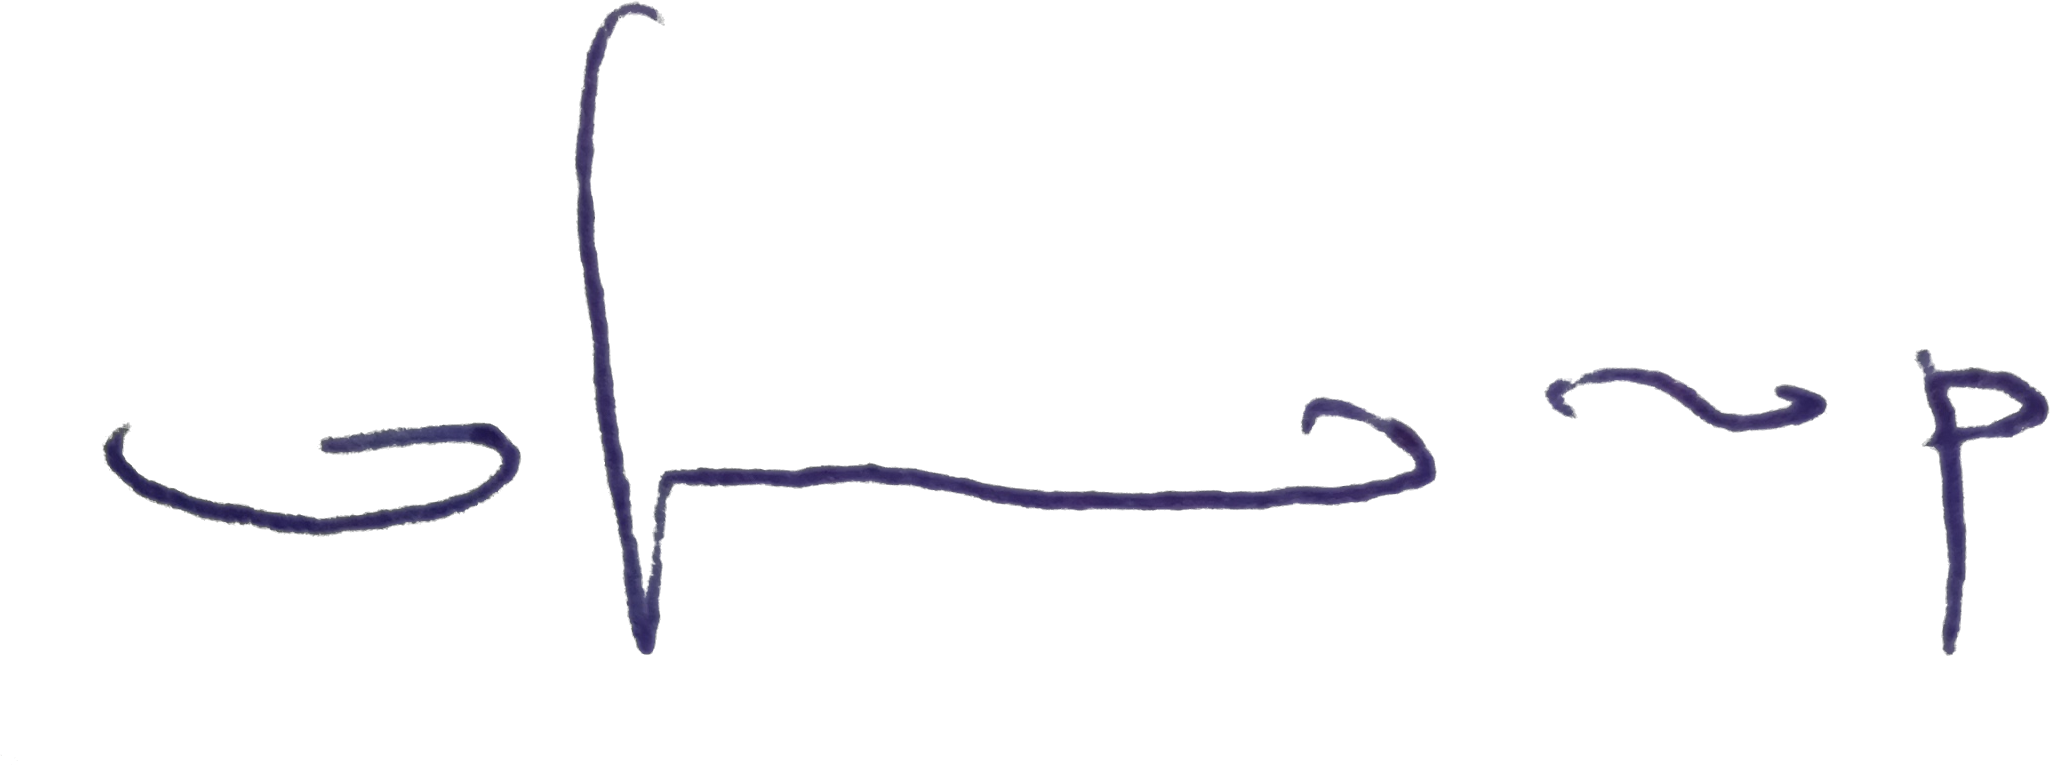
\includegraphics[width=4cm]{sig/garden.png}
    &
    Огородникова Ольга Михайловна
\end{tabularx}


\clearpage
